%! Author = thibaultchausson
%! Date = 23/07/2023



\subsection*{Descriptions des Reels}\label{subsec:descriptions-reels}
\addcontentsline{toc}{subsection}{Descriptions des Reels}



[L'\gls{AE} en réel ep.1]

\noindent Salut à toi jeune étudiant !

\noindent On démarre cette nouvelle année en te présentant la vie associative de l'\gls{UTBM} à travers différents réels !
\noindent Au programme, présentation de l'\gls{AE}, des élections du pôle des festivités et pleins d'autres choses !
\noindent N'hésite pas à venir à notre rencontre, nous poser tes questions ou proposer tes idées pour améliorer la vie étudiante.

\noindent À très vite !


[L'\gls{AE} en réel ep.2]

\noindent Envie de montrer ce que tu as dans le ventre et mettre tout le monde d'accord que toi et tes amis êtes les meilleurs ambianceurs de l'\gls{UTBM}? \emoji{man-dancing}\emoji{woman-dancing}

\noindent Alors n'attendez plus, venez vite vous inscrire en équipe dans les listes de la battle de soirée \emoji{partying-face}.

\noindent Toutes les informations sont dans la vidéo et le prochain post \emoji{star-struck} !

\noindent \emoji{warning} les étudiants en TC01 ne seront pas selectionnés pour les listes, on préfère que vous veniez profiter des soirées \emoji{winking-face}.

\noindent N'hésitez pas à poser en commentaire toutes vos questions !


\subsection*{Interface Instagram}\label{subsec:interface-instagram}
\addcontentsline{toc}{subsection}{Interface Instagram}

\begin{figure}[!h]
    \begin{center}
        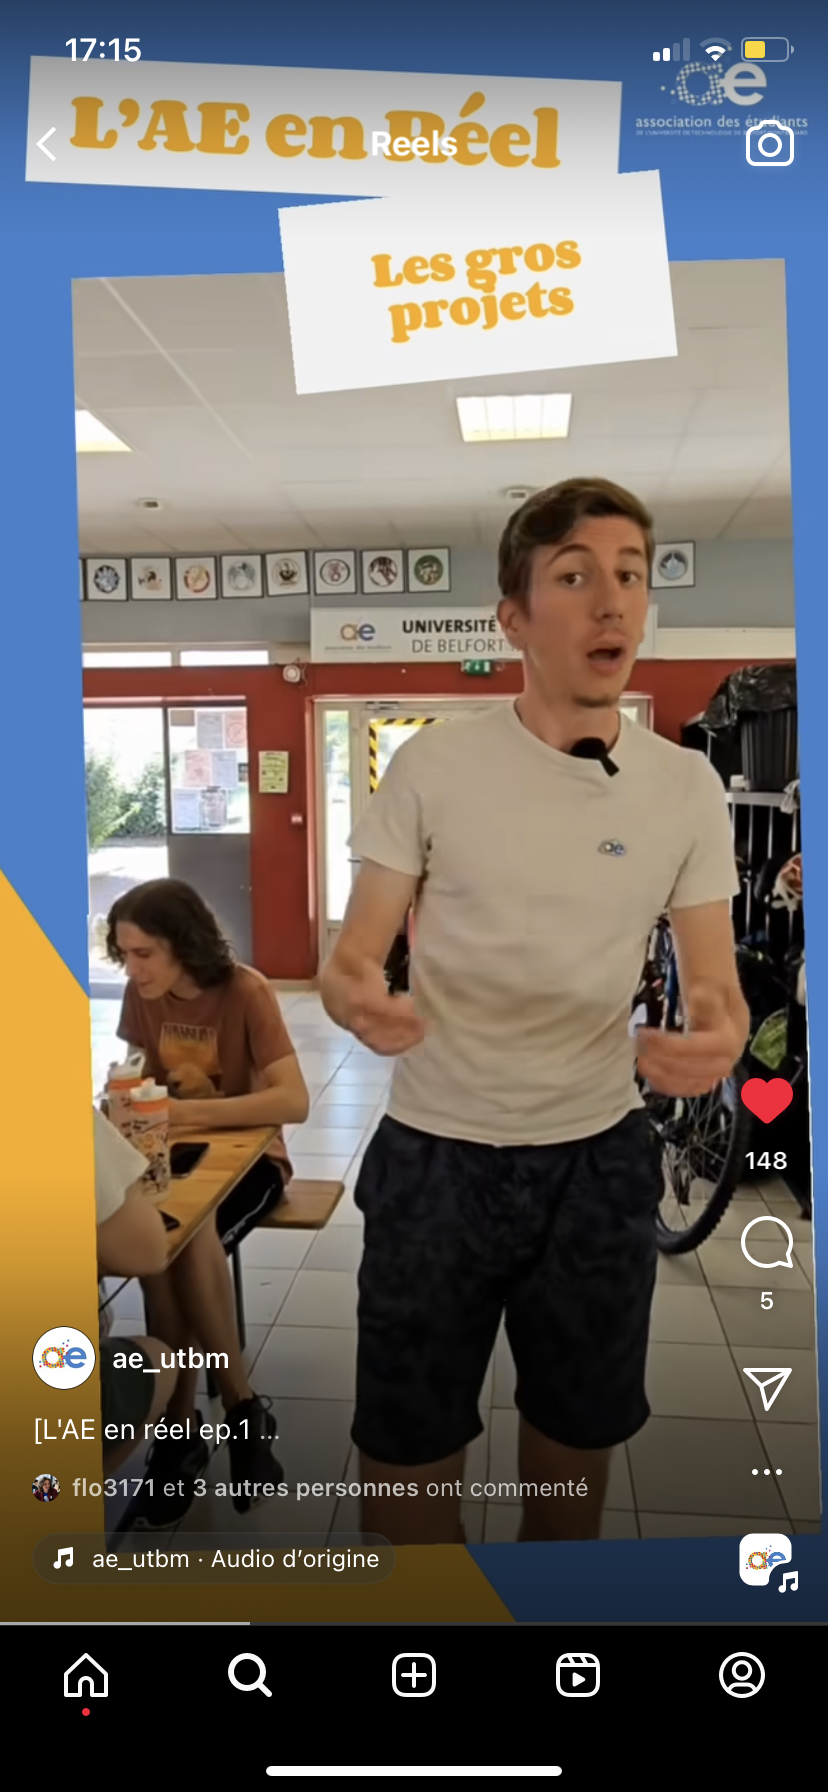
\includegraphics[scale=0.2]{ressources/interfaceInsta}
        \caption{Interface des Reels Instagram iOS \label{fig:interfaceInsta}}
    \end{center}
\end{figure}
